\documentclass{standalone}
\usepackage{tikz}
\usetikzlibrary{arrows}

\newcommand\reflexive[2]{% node, label
  \draw[->] (#1.100) to[reflexive] node[trans,above=-2mm] {#2} (#1.80);
}
\newcommand\link[3]{% start node, end node, label
  \draw[edge] (#1) -- (#1 |- #2);
  \node[trans] at (#1 |- #2) {#3} (1);
  \draw[edge] (#1 |- #2) -- (#2);
}
\newcommand\linkwithdots[4]{% start node, end node, dots node, label
  \coordinate (dots1) at (#1 |- #3);
  \draw (#1) -- ([yshift=5mm]dots1);
  \draw[dotted] ([yshift=5mm]dots1) -- ([yshift=-5mm]dots1);
  \draw[edge] ([yshift=-5mm]dots1) -- (#1 |- #2);
  \node[trans] at (#1 |- #2) {#4} (1);
  \coordinate (dots2) at (#3 |- #2);
  \draw (#1 |- #2) -- ([xshift=-5mm]dots2);
  \draw[dotted] ([xshift=-5mm]dots2) -- ([xshift=5mm]dots2);
  \draw[edge] ([xshift=5mm]dots2) -- (#2);
}
\begin{document}
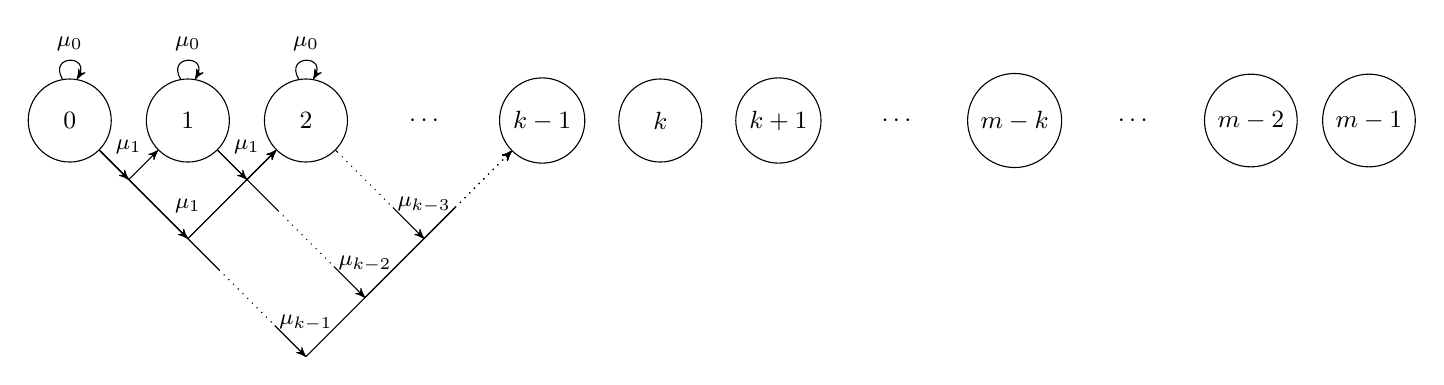
\begin{tikzpicture}
  \tikzset{
    >=stealth',
    node distance=1.5cm,
    state/.style={minimum size=30pt,font=\small,circle,draw},
    dots/.style={state,draw=none},
    edge/.style={->},
    trans/.style={font=\footnotesize,above=2mm},
    reflexive/.style={out=120,in=60,looseness=5,relative},
  }
  \node [state] (0)                    {$0$};
  \node [state] (1)   [right of = 0]   {$1$};
  \node [state] (2)   [right of = 1]   {$2$};
  \node [dots]  (d1)  [right of = 2]   {$\cdots$};
  \node [state] (km1) [right of = d1]  {$k-1$};
  \node [state] (k)   [right of = km1] {$k$};
  \node [state] (kp1) [right of = k]   {$k+1$};
  \node [dots]  (d2)  [right of = kp1] {$\cdots$};
  \node [state] (mmk) [right of = d2]  {$m-k$};
  \node [dots]  (d3)  [right of = mmk] {$\cdots$};
  \node [state] (mm2) [right of = d3]  {$m-2$};
  \node [state] (mm1) [right of = mm2] {$m-1$};

  \begin{scope}[rotate=45]
    \reflexive{0}{$\mu_0$}
    \reflexive{1}{$\mu_0$}
    \reflexive{2}{$\mu_0$}
    \link{0}{1}{$\mu_1$}
    \link{0}{2}{$\mu_1$}
    \link{1}{2}{$\mu_1$}
    \linkwithdots{0}{km1}{d1}{$\mu_{k-1}$}
    \linkwithdots{1}{km1}{d1}{$\mu_{k-2}$}
    \linkwithdots{2}{km1}{d1}{$\mu_{k-3}$}
  \end{scope}
\end{tikzpicture}
\end{document}
